%----------------------------------------------------------------------------
\chapter*{Az első lépések}\addcontentsline{toc}{chapter}{Az első lépések}
%----------------------------------------------------------------------------

\section{A környezet megismerése}

Ahhoz, hogy a fejelsztést meg tudjuk kezdeni szükségünk van néhány szoftverre, illetve a ZedBoard és a számítógép közötti megfelelő kapcsolat kialakítására. Az egyik legfontosabb szoftver a MATLAB és a Simulink. A MATLAB telepítése után fel kell telepítenünk a ZedBoard-hoz tartozó Hardvare Software Package-et. A telepítés folyamán a ZedBoardhoz tartozó SD kártyára egy speciális image-et is fel kell telepítenünk, ez automatikusan megtörténik. Miután készen vagyunk, csatlakoztatnunk kell a ZedBoard-ot a számítógépünkhöz. Ehhez szükség van egy Ethernet kábelre, illet kettő USB-kábelte, melyek a soros kommunikációt, illetve a JTAG kapcsolatot. A soros portra a kezdeti kapcsoalt miatt van szükség, a JTAG-re az FPGA megfelelő konfigurálásának érdekében, az Ethernetre pedig a szimuláció alatti gyors adatcsere miatt. 

\begin{figure}[!ht]
	\centering
	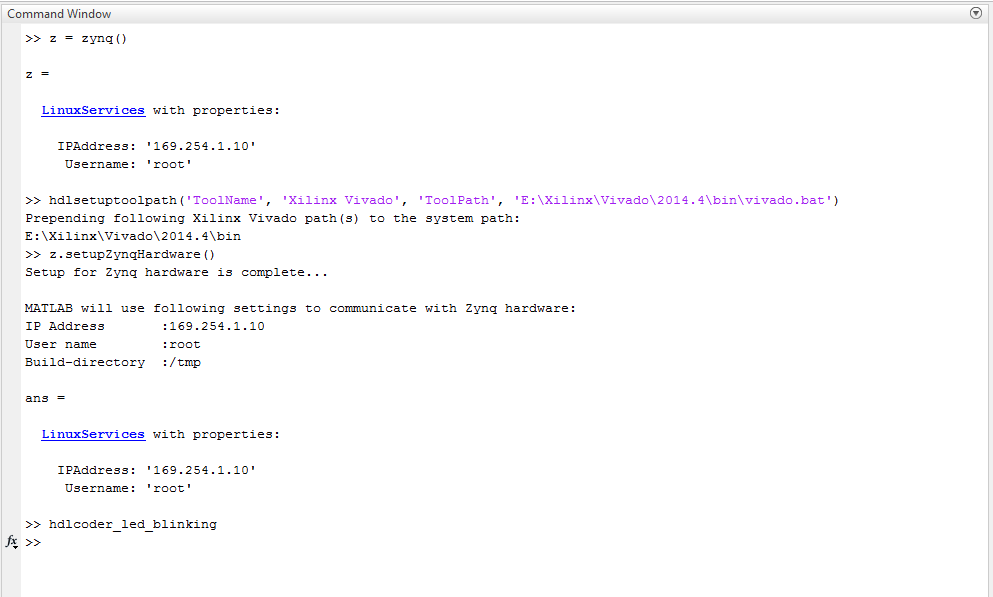
\includegraphics[width = \textwidth]{figures/matlab_1_setup.png}
	\caption{A MATLAB környezet konfigurálása} 
	\label{fig:matlabconf}
\end{figure}

Az alapvető működést egy egyszerű számláló segítségével mutatja be a dolgozat. Ennek modelljét \aref{fig:counter}, illetve \aref{fig:counter_sub} ábárn láthatjuk. \Aref{fig:counter} ábrán a bal oldalon találhatóak a felhasználó bemenetek, a jobb oldalon pedig két \emph{scope}, melyek segítségével megfigyelhetjük a kivezetett változókat, többke között pl. a számláló értékét. \Aref{fig:counter_sub} ábrán pedig a modell belső felépítése látható.

\begin{figure}[!ht]
	\centering
	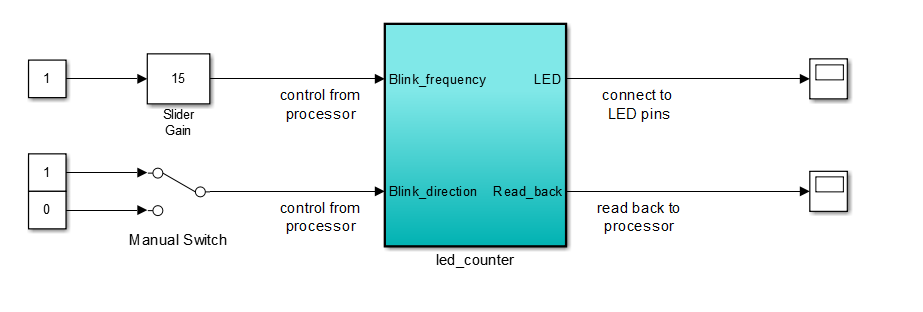
\includegraphics[width = \textwidth]{figures/simulink_1.png}
	\caption{A Simulinkben példa modell} 
	\label{fig:counter}
\end{figure}

Amennyiben a modellel elkészültünk, PC-n futtatva tesztelhetjük a megfelelő működést. Amenyiben elkészültünk, a HDL Workflow Advisor segítségével megkezdhetjük az FPGA projekt létrehozását. Fenti segédprogram végigkísér minket a szükséges lépéseken. Először meg kell adnunk, hogy milyen programmal, mit, és milyen eszközre akarunk készíteni. Jelen esetben a ZedBoard-ra akarunk készíteni egy IP Core-t, a Vivado programcsomaggal.

\begin{figure}[!ht]
	\centering
	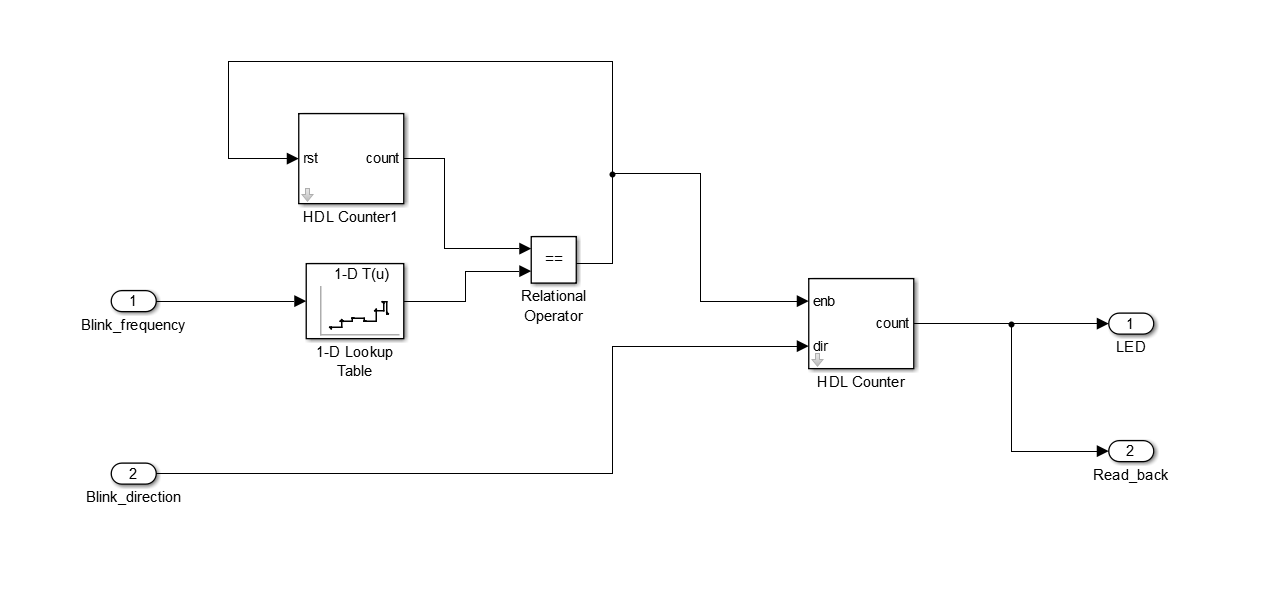
\includegraphics[width = \textwidth]{figures/counter.png}
	\caption{A Simulinkben megvalósított számláló} 
	\label{fig:counter_sub}
\end{figure}

A következő lépésben meg kell adni azt, hogy a fenti kapcsolatok hogyan fognak leképeződni az FPGA-ban fizikailag. A bementeinket egy \emph{AXI4-Lite} buszon keresztül fogjuk elérni. Ez egy kiválasztott címet jelent az SoC közös memóriájában, amire mi tudunk írni, illetve az FPGA blokk onnan olvassa be ezeket az adatokat. Az egyeteln dolog, amit nem így állítunk be, a a számláló, melynek értékét a panelen található LED-ekre is kivezetjük.

\begin{figure}[!ht]
	\centering
	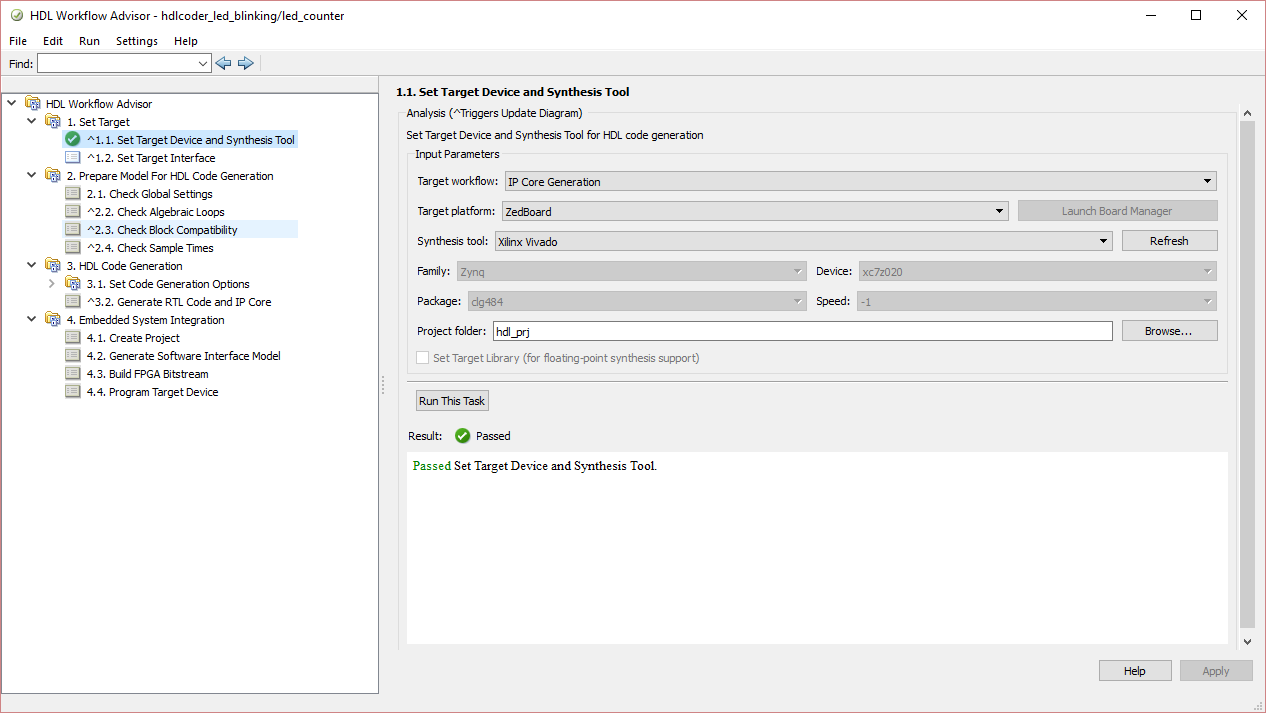
\includegraphics[width = \textwidth]{figures/hdlworkflow.PNG}
	\caption{A HDL kódgenerálás első lépése} 
	\label{fig:hdlgen}
\end{figure}


\begin{figure}[!ht]
	\centering
	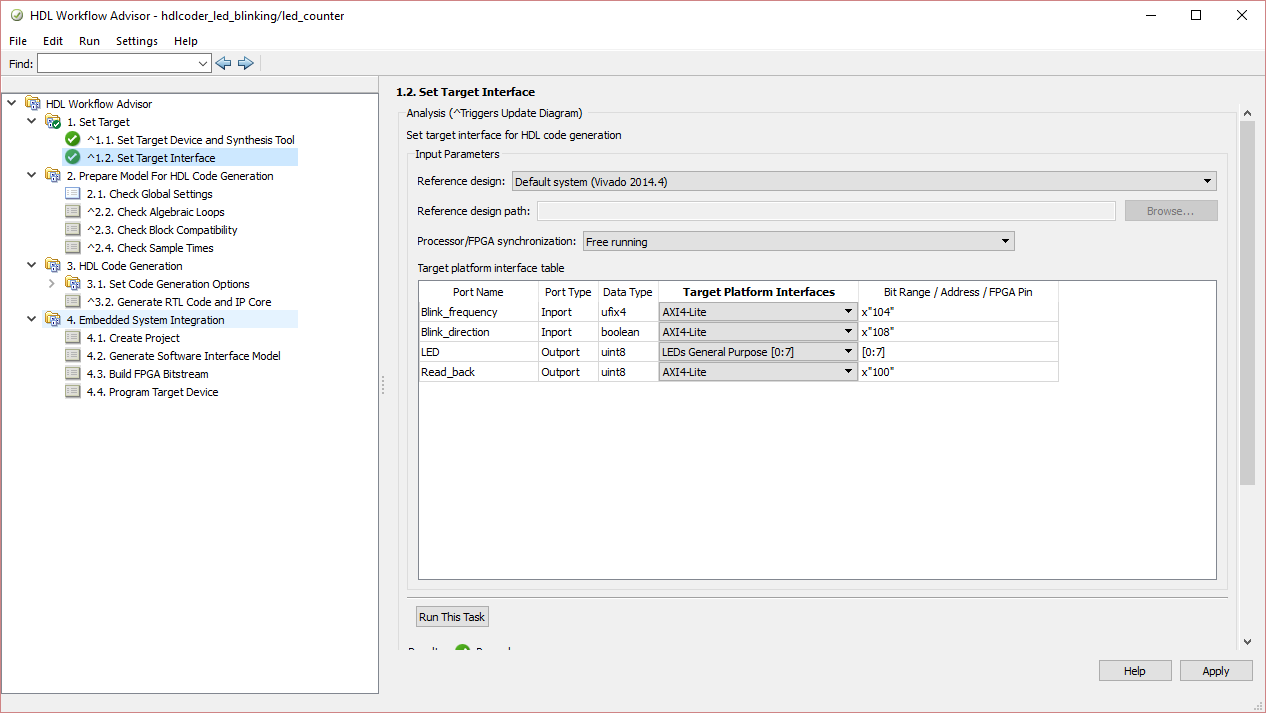
\includegraphics[width = \textwidth]{figures/hdl_2.PNG}
	\caption{A modell elemei és a valós perifériák összerendelése} 
	\label{fig:hdlgen_2}
\end{figure}

Miután ezzel kész vagyunk, a többi lépés gyakorlatilag teljesen automatikus, ezért lefuttathatjuk egyben. Elkészül a Vivado projekt, melynek lefordítására a MATLAB meghívja a Vivado környezetét, elkészíti a bitstreamet, illetve egy C compiler segítségével a modellből készít egy ún. Software Interface modellt. Később ennek segítségével tudjuk a elérni az FPGA-t


\begin{figure}[!ht]
	\centering
	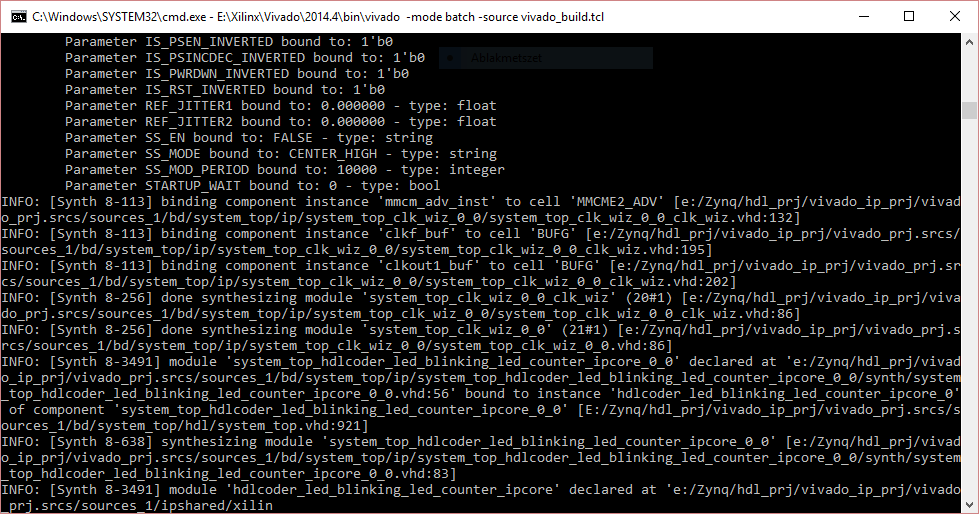
\includegraphics[width = \textwidth]{figures/bitstream.PNG}
	\caption{A HDL projekt fordításásnak kimenete} 
	\label{fig:bitstream}
\end{figure}

\begin{figure}[!ht]
	\centering
	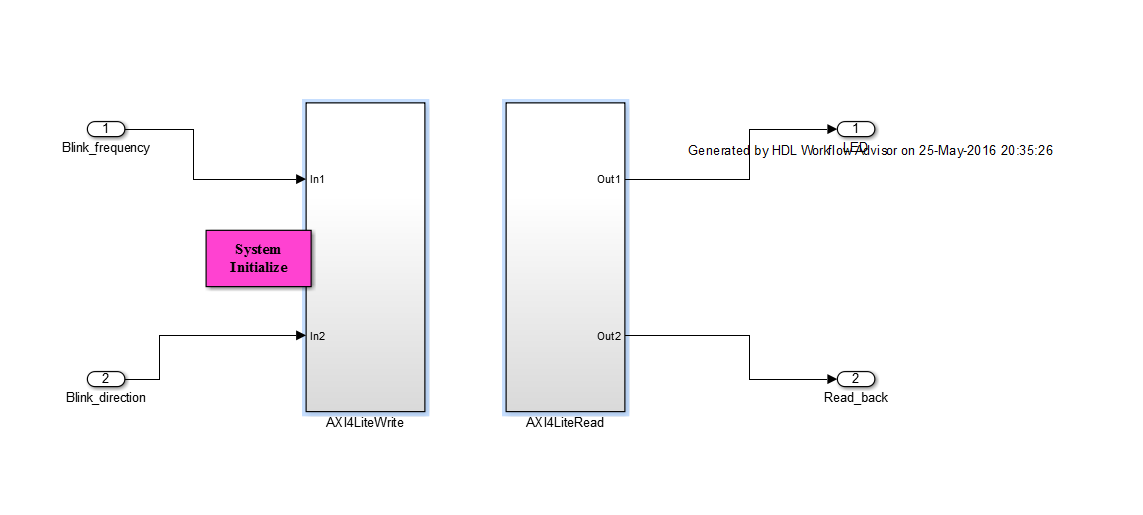
\includegraphics[width = \textwidth]{figures/interface.PNG}
	\caption{A generált Software interface modell} 
	\label{fig:swinterface}
\end{figure}

A Softvare Interface modell első ránézésre ugyan az a modell, mint amit mi készítettünk a folyamat elején. A különbség a színfalak mögött van, ha belenézünk a középső kék blokkba, akkor láthatjuk, hogy itt már nem a számláló van, hanem egy \emph{AXI4LiteWrite} és egy \emph{AXI4LiteRead} blokk található. Tehát a korábbi bemeneteink tényleg leredukálódtak memóriacímekre való írásra, és onnan való olvasásra.

Ahhoz, hogy az FPGA-van valóban kommunikálni tudjunk, ennek a modellnek a futásidejét állítsuk végtelenre, és indísuk el \emph{External} módban. Ez után tudjuk állítani a számlálási frekvenciát, irányt, illetve a kiementeket megnyitva láthatjuk a számláló által létrehozott fűrészjelet is.

\begin{figure}[!ht]
	\centering
	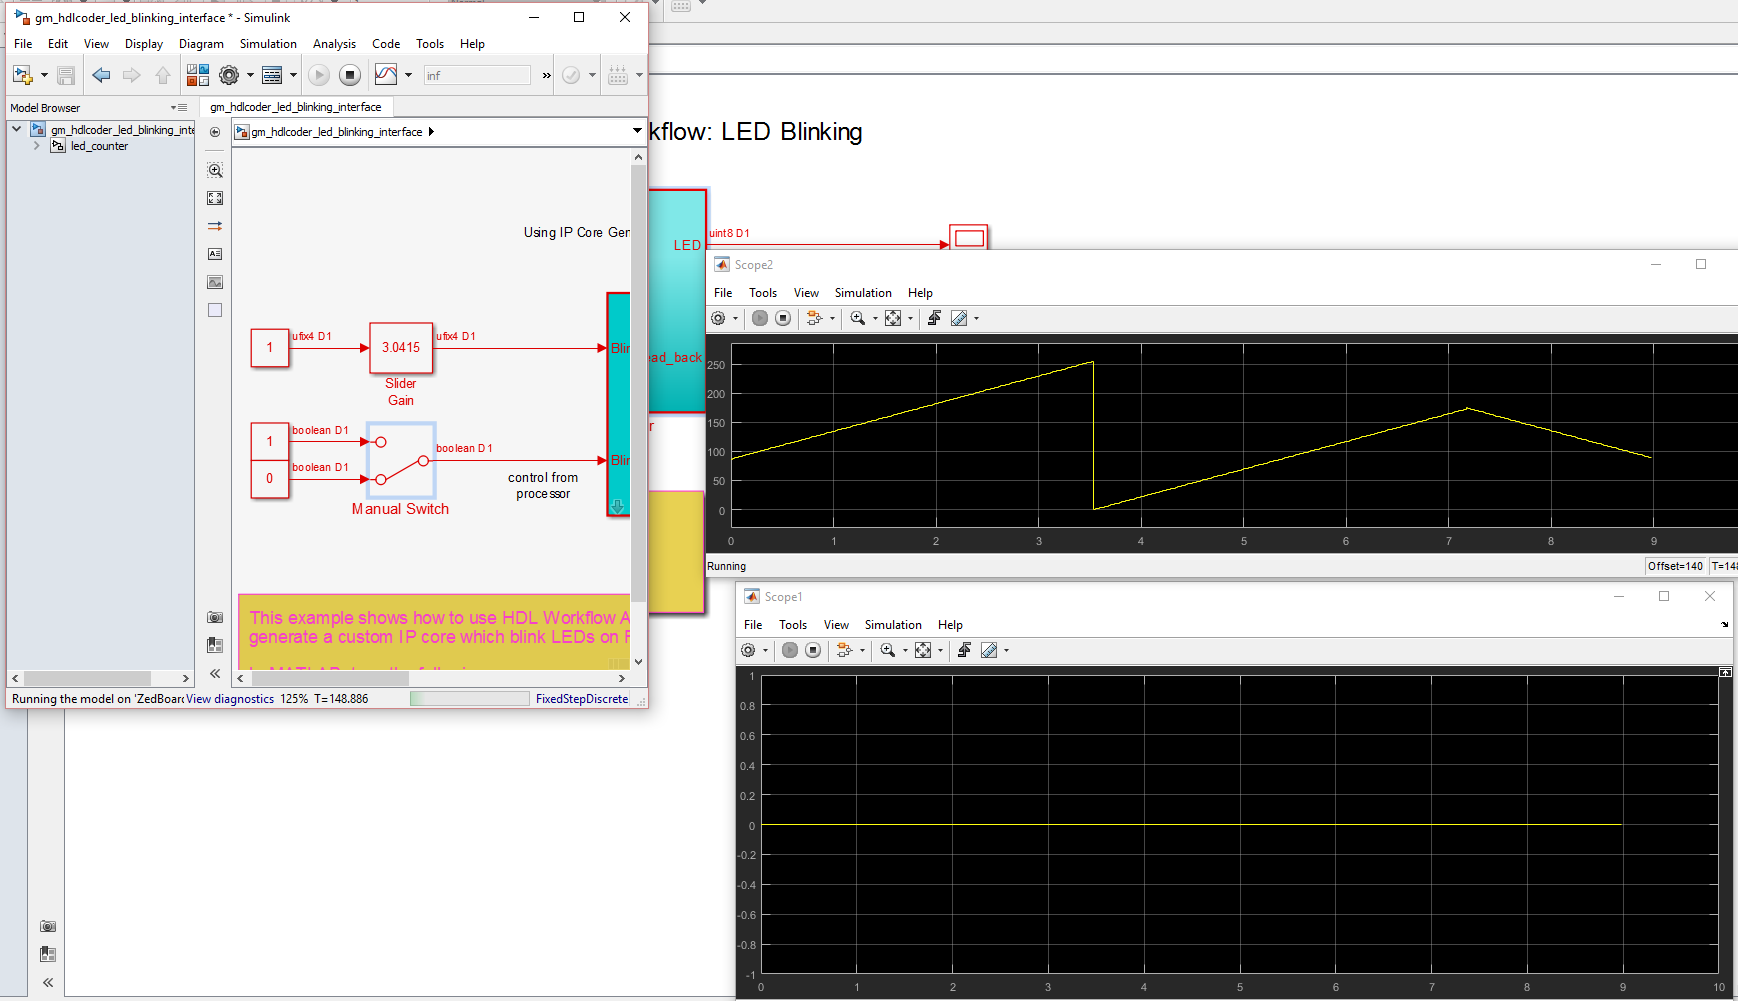
\includegraphics[width = \textwidth]{figures/running.PNG}
	\caption{A futó szimuláció} 
	\label{fig:simualtion}
\end{figure}